\documentclass[11pt]{amsart}

\usepackage[T1]{fontenc}
\usepackage{lmodern}
\usepackage{amssymb,amsmath}
\usepackage{graphicx}
\usepackage{booktabs}
\usepackage{xcolor}
\usepackage[margin=1.15in]{geometry}
\usepackage[colorlinks=true,linkcolor=blue!50!black,citecolor=blue!50!black,urlcolor=blue!50!black]{hyperref}

\newtheorem{theorem}{Theorem}[section]
\newtheorem{proposition}[theorem]{Proposition}
\newtheorem{lemma}[theorem]{Lemma}
\newtheorem{corollary}[theorem]{Corollary}
\theoremstyle{definition}
\newtheorem{definition}[theorem]{Definition}
\newtheorem{question}[theorem]{Question}
\theoremstyle{remark}
\newtheorem{remark}[theorem]{Remark}

\newcommand{\doi}[1]{\href{https://doi.org/#1}{\nolinkurl{doi:#1}}}
\newcommand{\SF}{\operatorname{SF}}
\hypersetup{pdftitle={Upper k-star-forming sets and k-independence in bipartite graphs},pdfauthor={Deep Bhattacharjee}}

\begin{document}

\title[Upper $k$-star-forming sets in bipartite graphs]{Upper $k$-star-forming sets and $k$-independence\\ in bipartite graphs}

\author{Deep Bhattacharjee}
\address{Formerly, Electro-Gravitational Space Propulsion Laboratory (EGSPL),\newline Bhubaneswar, Odisha 751030, India}
\email{d.bhattacharjee@erl-forschung.de}
\email{itsdeep@live.com}
\urladdr{https://orcid.org/0000-0003-0466-750X}
\thanks{Corresponding author: \href{mailto:d.bhattacharjee@erl-forschung.de}{d.bhattacharjee@erl-forschung.de}; ORCID \href{https://orcid.org/0000-0003-0466-750X}{\mbox{0000-0003-0466-750X}}}

\subjclass[2020]{Primary 05C69; Secondary 68Q17}
\keywords{$k$-independence, $k$-star-forming set, upper domination, bipartite graph, chain graph, NP-completeness, formal verification}

\begin{abstract}
Sahbi conjectured that the $k$-independence number $\beta_k$ and the upper $k$-star-forming number $\SF_k$ agree on bipartite graphs, and in particular on chain graphs, and asked whether $\beta_3=\SF_3$ on triangle-free graphs. For every $k\ge3$ we give a connected bipartite graph on $3k+3$ vertices with $\beta_k=2k+2$ and $\SF_k\ge3k$. On chain graphs, however, $\beta_k=\SF_k$ for every $k$. We also show, answering another of his questions, that deciding whether a bipartite graph has a minimal $2$-star-forming set with at least $t$ vertices is NP-complete.
\end{abstract}

\maketitle

\section{Introduction}

Let $G$ be a finite simple graph and $k$ a positive integer. A set $I$ of vertices is \emph{$k$-independent} if the induced subgraph $G[I]$ has maximum degree less than $k$, and $\beta_k(G)$ is the largest size of such a set; this notion goes back to Fink and Jacobson~\cite{FJ}, see the survey~\cite{CFHV} and~\cite{BCFM}. Chellali and Favaron~\cite{CF} called a set $S$ \emph{$k$-star-forming} if for every vertex $v\notin S$ the graph $G[S\cup\{v\}]$ contains a copy of the star $K_{1,k}$ that contains $v$, and they showed that $\beta_k(G)\le\SF_k(G)$, where $\SF_k(G)$ is the largest size of a minimal $k$-star-forming set.\footnote{A maximal $k$-independent set $I$ is $k$-star-forming, and it is minimal with that property, since a vertex $s\in I$ has fewer than $k$ neighbours in $I$ and so lies in no copy of $K_{1,k}$ inside $G[I]$.} For $k=1$ these are the independence number $\alpha$ and the upper domination number $\Gamma$, and the theorem of Cockayne, Favaron, Payan and Thomason~\cite{CFPT} that $\Gamma=\alpha$ for bipartite graphs is the first case of the following conjecture of Sahbi.\footnote{Sahbi withdrew the preprint~\cite{Sa} on 12 October 2026 with the comment ``Some conjectures in this paper have been disproved''. We refer to its second version.}

\begin{question}[{\cite[Conjecture~4.1]{Sa}}]
Is $\beta_k(G)=\SF_k(G)$ for every bipartite graph $G$ and every $k\ge1$?
\end{question}

Sahbi proved the equality for complete bipartite graphs and every $k$, and for chain graphs when $k=2$; he gave a triangle-free graph on ten vertices with $\beta_4<\SF_4$, and asked~\cite[Problem~7.3]{Sa} whether $\beta_3=\SF_3$ for every triangle-free graph. The case $k=2$ of the conjecture was refuted by a ten-vertex bipartite graph with $\beta_2=5$ and $\SF_2=6$, posted on 9 October 2026 to a public repository of refutations~\cite{OR}.\footnote{We checked this example and found by exhaustive search that it is the only bipartite graph with at most ten vertices and $\beta_2<\SF_2$ (Remark~\ref{rem:small}).} We show that the conjecture fails for every larger $k$ as well.

\begin{theorem}\label{thm:main}
For every $k\ge3$ the connected bipartite graph $G_k$ of Section~\ref{sec:graph}, on $3k+3$ vertices, satisfies
\[
\beta_k(G_k)=2k+2\qquad\text{and}\qquad \SF_k(G_k)\ge3k.
\]
\end{theorem}

In particular $\SF_k(G_k)-\beta_k(G_k)\ge k-2$, and the answer to Problem~7.3 of~\cite{Sa} is negative already for bipartite graphs: $G_3$ has twelve vertices and $\beta_3(G_3)=8<9\le\SF_3(G_3)$. Together with the example for $k=2$, the equality $\beta_k=\SF_k$ holds on all bipartite graphs only for $k=1$, which answers Sahbi's Problem~9.4 for the class of bipartite graphs.

The equality does survive on the more rigid class of chain graphs, the bipartite graphs in which the neighbourhoods of the vertices on one side are nested. Sahbi proved $\beta_2=\SF_2$ for chain graphs and conjectured~\cite[Conjecture~6.4]{Sa} that $\beta_k=\SF_k$ for chain graphs and all $k\ge3$; this is his Problem~9.1. We prove it.

\begin{theorem}\label{thm:chain}
For every chain graph $G$ and every $k\ge2$, $\beta_k(G)=\SF_k(G)$.
\end{theorem}

The proof in Section~\ref{sec:chain} shows that in a chain graph a minimal $k$-star-forming set has at most one vertex with $k$ or more neighbours inside it, and that this vertex can be exchanged for a vertex outside the set. The graphs $G_k$ show that some such rigidity is needed: in $G_k$ all $k-1$ hubs have $2k-1$ neighbours in the set $S$ of Lemma~\ref{lem:S}.

Sahbi also asked~\cite[Problem~9.3]{Sa} for the complexity of computing $\SF_2$ on bipartite graphs, and in particular whether it is NP-complete to decide, for a bipartite graph $G$ and an integer $t$, whether $G$ has a minimal $2$-star-forming set with at least $t$ vertices. It is. For a graph $H$ let $H^\sharp$ be the graph obtained from $H$ by replacing every edge with a path of length four and attaching a pendant vertex to every vertex of $H$ (Section~\ref{sec:np}).

\begin{theorem}\label{thm:np}
Let $H$ be a graph with $n$ vertices, $m$ edges and independence number $\alpha(H)$. Then $H^\sharp$ is a bipartite graph on $2n+3m$ vertices, and
\[
\beta_2(H^\sharp)=\SF_2(H^\sharp)=n+2m+\alpha(H).
\]
Hence it is NP-complete to decide whether a bipartite graph has a minimal $2$-star-forming set with at least $t$ vertices, and this remains so for planar bipartite graphs.
\end{theorem}

The graphs $H^\sharp$ satisfy Sahbi's equality, so the hardness does not come from a gap between the two numbers. The same identity gives another proof that computing $\beta_2$, the dissociation number, is NP-hard on bipartite graphs, a result of Yannakakis~\cite{Ya}.

\section{The graphs \texorpdfstring{$G_k$}{G\_k}}\label{sec:graph}

We write $N_S(v)$ for the set of neighbours of $v$ in $S$ and $d_S(v)=|N_S(v)|$. A copy of $K_{1,k}$ in $G[S\cup\{v\}]$ containing $v\notin S$ has $v$ as its centre or as a leaf, which gives the following local form of the definition~\cite[Lemma~2.2]{Sa}.

\begin{lemma}\label{lem:local}
A set $S$ is $k$-star-forming if and only if every vertex $v\notin S$ satisfies $d_S(v)\ge k$ or has a neighbour $u\in S$ with $d_S(u)\ge k-1$. Every superset of a $k$-star-forming set is $k$-star-forming, so a $k$-star-forming set $S$ is minimal if and only if $S\setminus\{s\}$ is not $k$-star-forming for each $s\in S$.
\end{lemma}

Fix $k\ge2$. The graph $G_k$ has the $3k+3$ vertices
\[
h_1,\dots,h_{k-1},\qquad u_1,\dots,u_{k-1},\qquad w_1,\dots,w_{k-1},\qquad x_0,\ p,\ c_1,\ c_2,\ q_1,\ q_2 .
\]
Write $H=\{h_1,\dots,h_{k-1}\}$ for the \emph{hubs}, $X_1=\{u_1,\dots,u_{k-1}\}$, $X_2=\{w_1,\dots,w_{k-1}\}$ and $X=X_1\cup X_2\cup\{x_0\}$. The edges are
\begin{itemize}
\item $h_ix$ for every hub $h_i$ and every $x\in X$;
\item $x_0p$, $\ c_1q_1$ and $c_2q_2$;
\item $c_1u_j$ and $c_2w_j$ for $1\le j\le k-1$.
\end{itemize}
So $G_k$ has $(k-1)(2k-1)+2(k-1)+3=2k^2-k+2$ edges. It is connected, and it is bipartite with parts $H\cup\{p,c_1,c_2\}$ and $X\cup\{q_1,q_2\}$. Figure~\ref{fig:G3} shows $G_3$, which has $12$ vertices and $17$ edges.

\begin{figure}[t]
\centering
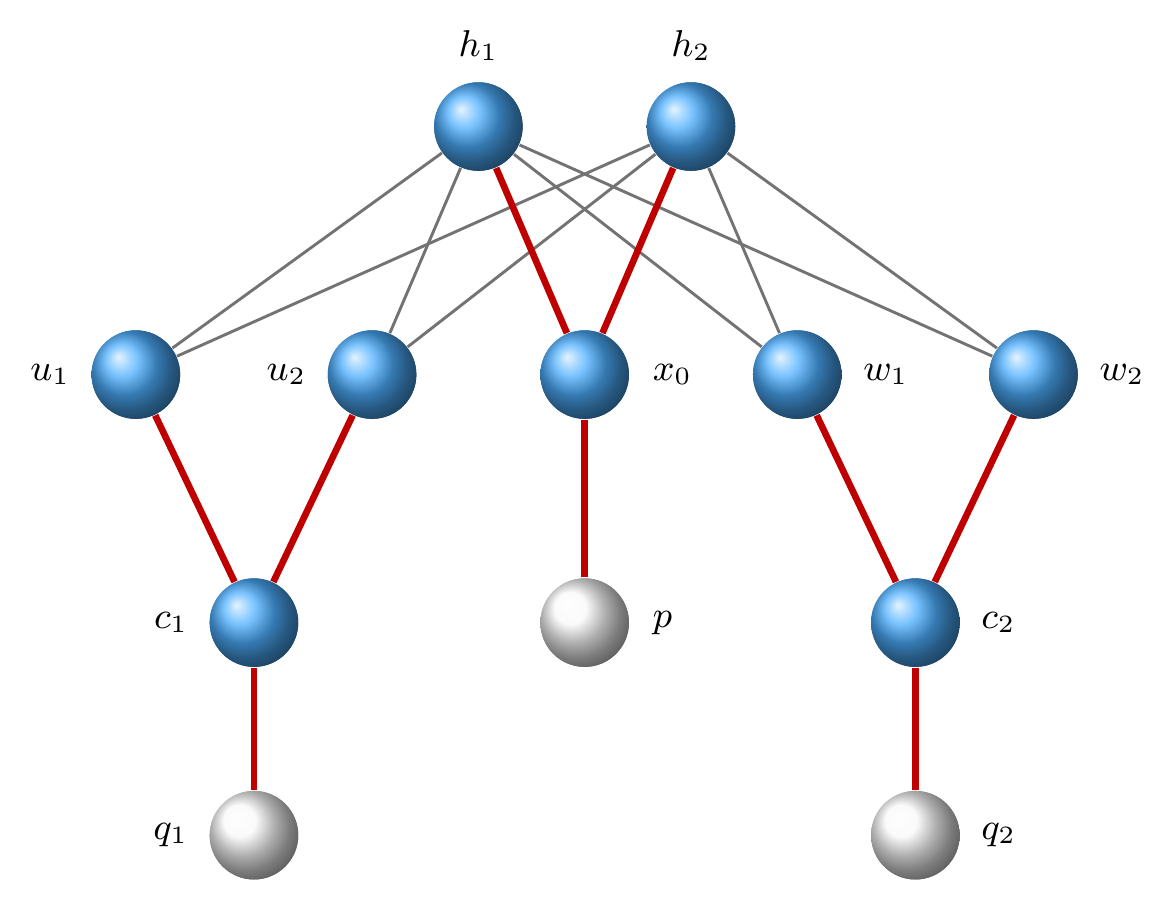
\includegraphics[width=0.56\textwidth]{figures/g3.png}
\caption{The graph $G_3$. The nine shaded vertices form a minimal $3$-star-forming set $S$, while every $3$-independent set has at most eight vertices. The thick edges are the three stars $K_{1,3}$ that place $p$, $q_1$ and $q_2$ in stars over $S$.}\label{fig:G3}
\end{figure}

The vertices $x_0$, $c_1$ and $c_2$ each see exactly $k-1$ vertices of $H\cup X$: the hubs, the block $X_1$ and the block $X_2$, respectively. Each of them also carries a pendant vertex, and the three pendant vertices $p$, $q_1$, $q_2$ are left outside the set $S$ below. Each pendant vertex is a leaf of a star whose centre and other leaves are forced into $S$, and this is what makes $S$ minimal although $S$ is far from $k$-independent: a hub has $2k-1$ neighbours in $S$.

\section{Proof of Theorem~\ref{thm:main}}

\begin{lemma}\label{lem:S}
For $k\ge2$ the set $S=V(G_k)\setminus\{p,q_1,q_2\}$ is a minimal $k$-star-forming set of $G_k$ with $|S|=3k$.
\end{lemma}

\begin{proof}
Clearly $|S|=3(k-1)+3=3k$. In $S$ we have $N_S(x_0)=H$, $N_S(c_1)=X_1$ and $N_S(c_2)=X_2$, so $d_S(x_0)=d_S(c_1)=d_S(c_2)=k-1$. The only vertices outside $S$ are $p$, $q_1$, $q_2$, and their neighbours $x_0$, $c_1$, $c_2$ lie in $S$; by Lemma~\ref{lem:local}, $S$ is $k$-star-forming.

For minimality we use Lemma~\ref{lem:local} again. The pendant vertices have degree $1<k$, so after the deletion of a vertex $s$ from $S$ a pendant vertex is still in a star only if its unique neighbour remains in $S\setminus\{s\}$ with at least $k-1$ neighbours there. If $s$ is a hub, then $x_0$ keeps only $k-2$ neighbours, so $p$ lies in no star. If $s=x_0$, then $p$ has no neighbour left. Likewise deleting a vertex of $X_1$, or $c_1$, leaves $q_1$ outside every star, and deleting a vertex of $X_2$, or $c_2$, does the same to $q_2$. These cases cover all of $S$.
\end{proof}

\begin{lemma}\label{lem:beta}
For $k\ge2$, $\beta_k(G_k)=2k+2$.
\end{lemma}

\begin{proof}
The set $I_0=X\cup\{p,q_1,q_2\}$ induces the single edge $x_0p$ together with isolated vertices, so it is $k$-independent, and $|I_0|=2(k-1)+1+3=2k+2$.

Conversely, let $I$ be $k$-independent and put $t=|I\cap H|$ and $s=|I\cap X|$. If $t=0$, then $I$ lies in $G_k-H$, which is the disjoint union of the edge $x_0p$ and the two stars with centres $c_1$, $c_2$ and leaf sets $X_1\cup\{q_1\}$, $X_2\cup\{q_2\}$, each a copy of $K_{1,k}$. A $k$-independent set meets $K_{1,k}$ in at most $k$ vertices, since if it contains the centre it must omit a leaf; hence $|I|\le2+k+k$.

Suppose $t\ge1$. A hub in $I$ is adjacent to every vertex of $I\cap X$, so $s\le k-1$. Besides $H$ and $X$, at most the five vertices $p,c_1,c_2,q_1,q_2$ remain, so $|I|\le t+s+5$, which is at most $2k+2$ when $t\le k-2$. Finally let $t=k-1$. Every $x\in I\cap X$ is adjacent to all $k-1$ hubs, all of which lie in $I$, so its remaining neighbour among $p$, $c_1$, $c_2$ (namely $p$ for $x_0$, $c_1$ on $X_1$ and $c_2$ on $X_2$) is not in $I$. If $s\ge1$ this removes at least one of $p,c_1,c_2$, and $|I|\le(k-1)+(k-1)+2+2=2k+2$. If $s=0$, then $|I|\le(k-1)+5\le2k+2$.
\end{proof}

\begin{proof}[Proof of Theorem~\ref{thm:main}]
By Lemma~\ref{lem:S}, $\SF_k(G_k)\ge|S|=3k$, and by Lemma~\ref{lem:beta}, $\beta_k(G_k)=2k+2$, which is smaller than $3k$ once $k\ge3$.
\end{proof}

\section{Chain graphs}\label{sec:chain}

Let $G$ be a chain graph with parts $A$ and $B$, so that the neighbourhoods $N(a)$, $a\in A$, form a chain under inclusion. Then the neighbourhoods $N(b)$, $b\in B$, form a chain as well.\footnote{If $a\in N(b)\setminus N(b')$ and $a'\in N(b')\setminus N(b)$, then $b\in N(a)\setminus N(a')$ and $b'\in N(a')\setminus N(a)$, so $N(a)$ and $N(a')$ are incomparable.} Two vertices on the same side therefore satisfy $N(u)\subseteq N(v)$ or $N(v)\subseteq N(u)$, and $N(u)\subseteq N(v)$ implies $d_S(u)\le d_S(v)$ for every set $S$. We say that $S$ \emph{covers} a vertex $v\notin S$ if $v$ satisfies the condition of Lemma~\ref{lem:local}. Deleting a vertex $s$ from $S$ changes $d_S$ only on the neighbours of $s$, which lie on the other side.

The exchange step works in every graph.

\begin{lemma}\label{lem:exchange}
Let $S$ be a minimal $k$-star-forming set of a graph $G$, $k\ge1$, such that at most one vertex $v\in S$ has $d_S(v)\ge k$. Then $\beta_k(G)\ge|S|$.
\end{lemma}

\begin{proof}
If no vertex of $S$ has $d_S(v)\ge k$, then $S$ itself is $k$-independent. Otherwise let $h$ be the vertex with $d_S(h)\ge k$. By Lemma~\ref{lem:local} some vertex $z\notin S\setminus\{h\}$ is not covered by $S\setminus\{h\}$: it has at most $k-1$ neighbours in $S\setminus\{h\}$, and each of these has at most $k-2$ neighbours in $S\setminus\{h\}$. As $h$ has $d_S(h)\ge k$ neighbours in $S\setminus\{h\}$, we have $z\ne h$, so $z\notin S$. In $I=(S\setminus\{h\})\cup\{z\}$ the vertex $z$ has at most $k-1$ neighbours, each neighbour of $z$ has at most $(k-2)+1$, and every other vertex $v$ has at most $d_S(v)\le k-1$, since $v\ne h$. Hence $I$ is $k$-independent, and $|I|=|S|$.
\end{proof}

\begin{lemma}\label{lem:otherside}
Let $G$ be a chain graph, $k\ge2$, and $S$ a minimal $k$-star-forming set. If $h\in S$ has $d_S(h)\ge k$, then $d_S(y)\le k-2$ for every $y\in S$ on the other side.
\end{lemma}

\begin{proof}
We first show that every neighbour $y$ of $h$ in $S$ has a neighbour $w\notin S$ such that $d_S(u)\le k-2$ for every neighbour $u\ne y$ of $w$ in $S$. Some vertex $w\notin S\setminus\{y\}$ is not covered by $S\setminus\{y\}$. It is not $y$, since $h$ is a neighbour of $y$ with $d_S(h)-1\ge k-1$ neighbours in $S\setminus\{y\}$; so $w\notin S$, and $S$ covers $w$. Suppose $w$ lies on the side of $y$. Then $w$ is not adjacent to $y$, so $d_S(w)=d_{S\setminus\{y\}}(w)<k$, and $w$ has a neighbour $u\in S$ with $d_S(u)\ge k-1$, and $u$ lies on the side of $h$. If $N(u)\subseteq N(h)$, then $h$ is a neighbour of $w$ with at least $k-1$ neighbours in $S\setminus\{y\}$; if $N(h)\subseteq N(u)$, then $d_S(u)\ge d_S(h)\ge k$ and $u$ keeps at least $k-1$ neighbours in $S\setminus\{y\}$. Either way $S\setminus\{y\}$ covers $w$, which is impossible. So $w$ lies on the side of $h$, and its neighbours, lying on the side of $y$, have the same degree in $S\setminus\{y\}$ as in $S$. If $w$ were not adjacent to $y$, it would also keep its own degree, and $S\setminus\{y\}$ would cover $w$ as $S$ does. Hence $w$ is adjacent to $y$, and since $S\setminus\{y\}$ does not cover $w$, every neighbour $u\ne y$ of $w$ in $S$ has $d_S(u)\le k-2$.

Now $h$ has two neighbours $a\ne b$ in $S$, and we may assume $N(a)\subseteq N(b)$. Let $w$ be the vertex just found for $a$. Then $w$ is adjacent to $b$, so $d_S(b)\le k-2$. Let $y\in S$ lie on the side of $a$ and $b$. If $N(y)\subseteq N(b)$, then $d_S(y)\le d_S(b)\le k-2$. If $N(b)\subseteq N(y)$, then $w$ is adjacent to $y$, so $d_S(y)\le k-2$ when $y\ne a$, while $d_S(a)\le d_S(b)$.
\end{proof}

\begin{lemma}\label{lem:unique}
Let $G$ be a chain graph, $k\ge2$, and $S$ a minimal $k$-star-forming set. At most one vertex $v\in S$ has $d_S(v)\ge k$.
\end{lemma}

\begin{proof}
Suppose that $h\ne t$ are two such vertices. By Lemma~\ref{lem:otherside} they lie on the same side, and we may assume $N(t)\subseteq N(h)$. Some vertex $z\notin S\setminus\{t\}$ is not covered by $S\setminus\{t\}$, and $z\ne t$ since $d_{S\setminus\{t\}}(t)=d_S(t)\ge k$. So $z\notin S$, and $S$ covers $z$. If $z$ lies on the side of $t$, then $z$ is not adjacent to $t$, so $d_S(z)=d_{S\setminus\{t\}}(z)<k$, and $z$ has a neighbour $u\in S$ with $d_S(u)\ge k-1$; but $u$ lies on the other side from $h$, and $d_S(u)\le k-2$ by Lemma~\ref{lem:otherside}. If $z$ lies on the other side, then $z$ is not adjacent to $h$, which has $d_S(h)\ge k$ neighbours in $S\setminus\{t\}$; hence $z$ is not adjacent to $t$ either, as $N(t)\subseteq N(h)$. Then neither $z$ nor any of its neighbours, which lie on the side of $t$, changes its degree when $t$ is deleted, and $S\setminus\{t\}$ covers $z$ as $S$ does. Both cases are impossible.
\end{proof}

\begin{proof}[Proof of Theorem~\ref{thm:chain}]
We have $\beta_k(G)\le\SF_k(G)$ by~\cite{CF}. Conversely, every minimal $k$-star-forming set $S$ satisfies $|S|\le\beta_k(G)$ by Lemmas~\ref{lem:unique} and~\ref{lem:exchange}.
\end{proof}

For $k=1$ the equality holds on all bipartite graphs~\cite{CFPT}; the argument above needs $k\ge2$, since in Lemma~\ref{lem:otherside} the vertex $h$ must have two neighbours in $S$.

\section{Complexity}\label{sec:np}

Let $H$ be a graph with vertex set $V$, $n$ vertices and $m$ edges, and write each edge as an ordered pair $e=(u_e,v_e)$ of its ends, in either order. The graph $H^\sharp$ has the vertices of $H$, a new vertex $v'$ for every $v\in V$ and three new vertices $a_e,b_e,c_e$ for every edge $e$. Its edges are $vv'$ for $v\in V$ and the four edges of the path $u_e\,a_e\,b_e\,c_e\,v_e$ for every edge $e$ of $H$. So $H^\sharp$ has $2n+3m$ vertices; it is bipartite with parts $V\cup\{b_e\}$ and $\{v'\}\cup\{a_e,c_e\}$, and it is planar when $H$ is. Figure~\ref{fig:sharp} shows $K_3^\sharp$.

\begin{figure}[ht]
\centering
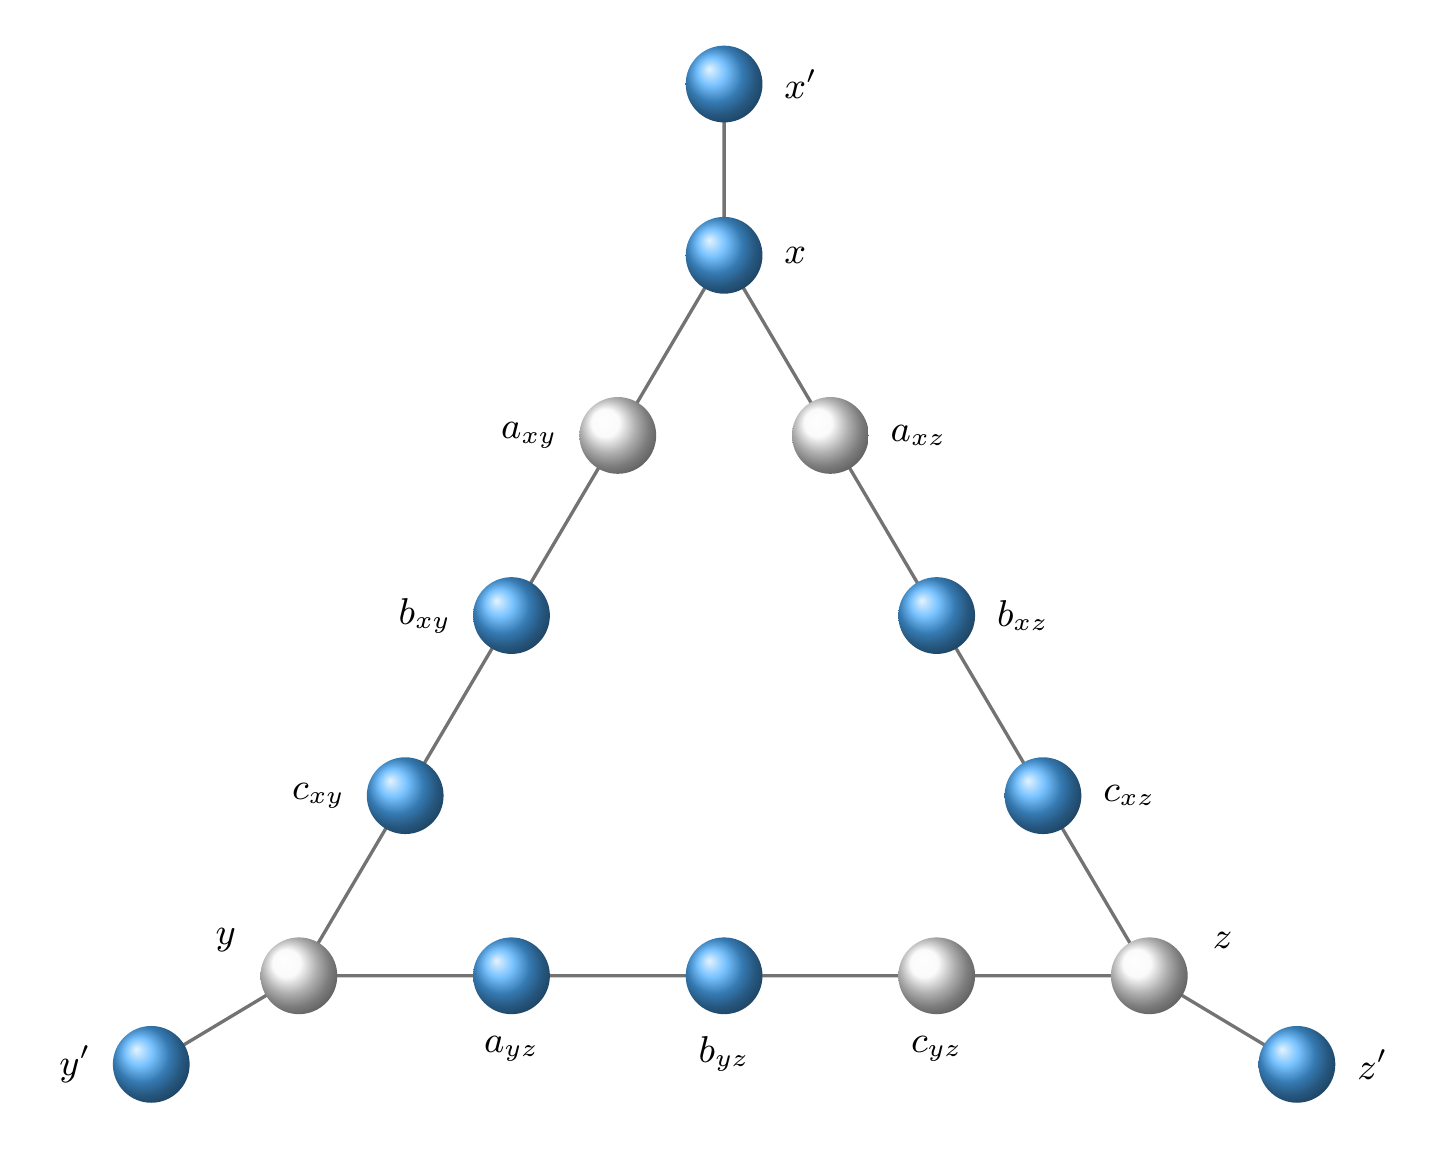
\includegraphics[width=0.5\textwidth]{figures/k3sharp.png}
\caption{The graph $K_3^\sharp$, with the edges ordered as $(x,y)$, $(y,z)$, $(x,z)$. The ten shaded vertices form the set $J(\{x\})$ of Lemma~\ref{lem:J}. It is a largest $2$-independent set and a largest minimal $2$-star-forming set, and $10=n+2m+\alpha(K_3)$.}\label{fig:sharp}
\end{figure}

\begin{lemma}\label{lem:J}
For every independent set $I$ of $H$ the set
\[
J(I)=I\cup\{v':v\in V\}\cup\{b_e:e\in E(H)\}\cup\{a_e:u_e\notin I\}\cup\{c_e:u_e\in I\}
\]
is $2$-independent in $H^\sharp$ and has $n+2m+|I|$ vertices.
\end{lemma}

\begin{proof}
The size is clear, since $J(I)$ contains exactly one of $a_e$ and $c_e$ for each edge $e$. We check that every vertex of $J(I)$ has at most one neighbour in $J(I)$. A vertex $v'$ has only one neighbour, and $b_e$ has exactly one of its neighbours $a_e,c_e$ in $J(I)$. Let $v\in I$. For an edge $e$ with $u_e=v$ the set $J(I)$ contains $c_e$ and not $a_e$, and for an edge $e$ with $v_e=v$ we have $u_e\notin I$, because $I$ is independent, so $J(I)$ contains $a_e$ and not $c_e$; hence $v'$ is the only neighbour of $v$ in $J(I)$. If $a_e\in J(I)$, then $u_e\notin I$, so $b_e$ is its only neighbour in $J(I)$. If $c_e\in J(I)$, then $u_e\in I$, so $v_e\notin I$, and again $b_e$ is its only neighbour in $J(I)$.
\end{proof}

For the upper bound we use Lemma~\ref{lem:local} with $k=2$: a set $S$ covers $w\notin S$ if $d_S(w)\ge2$ or $w$ has a neighbour $x\in S$ with $d_S(x)\ge1$. Let $s\in S$. If a vertex $w\notin S$ is neither adjacent to $s$ nor at distance two from it, then $d_{S\setminus\{s\}}(w)=d_S(w)$, and every neighbour $x$ of $w$ satisfies $x\ne s$ and $d_{S\setminus\{s\}}(x)=d_S(x)$, so $S\setminus\{s\}$ covers $w$ whenever $S$ does. Hence, to see that $S\setminus\{s\}$ is still $2$-star-forming, we only have to check $s$ and the vertices outside $S$ within distance two of $s$.

\begin{lemma}\label{lem:Ssharp}
Let $S$ be a minimal $2$-star-forming set of $H^\sharp$, and let $Y$ be the set of vertices $v\in V$ with $v\in S$ and $v'\in S$.
\begin{enumerate}
\item[(a)] Every $v\in V$ satisfies $v\in S$ or $v'\in S$.
\item[(b)] For no edge $e$ do all three of $a_e,b_e,c_e$ lie in $S$.
\item[(c)] If both ends of an edge $e$ lie in $Y$, then at most one of $a_e,b_e,c_e$ lies in $S$.
\end{enumerate}
\end{lemma}

\begin{proof}
(a) The vertex $v'$ has the single neighbour $v$, so if $v'\notin S$ then $S$ covers $v'$ only through $v\in S$.

(b) Suppose that $a_e,b_e,c_e\in S$, and put $S'=S\setminus\{b_e\}$. The vertex $b_e$ has its two neighbours $a_e$, $c_e$ in $S'$. The vertices outside $S$ at distance two from $b_e$ are among $u_e$ and $v_e$. If $u_e\notin S$, then $u_e'\in S$ by~(a), so $u_e$ has the two neighbours $u_e'$ and $a_e$ in $S'$, and likewise for $v_e$. So $S'$ is $2$-star-forming, against the minimality of $S$.

(c) Let $u_e,v_e\in Y$ and suppose that two of $a_e,b_e,c_e$ lie in $S$; by~(b) the third does not. Since $u_e'\in S$ and $v_e'\in S$, the vertices $u_e$ and $v_e$ keep at least one neighbour in $S$ after the deletion of any of $a_e,b_e,c_e$, so every vertex outside $S$ that is adjacent to $u_e$ or $v_e$ stays covered. If $b_e\notin S$, put $S'=S\setminus\{a_e\}$: then $a_e$ is covered through $u_e$, and $b_e$ through $c_e$, whose neighbour $v_e$ is in $S'$. If $c_e\notin S$, put $S'=S\setminus\{a_e\}$: then $a_e$ is covered through $u_e$, and $c_e$ has the two neighbours $b_e$ and $v_e$ in $S'$. The case $a_e\notin S$ is symmetric to the previous one, with $S'=S\setminus\{c_e\}$. In each case the vertices outside $S$ within distance two of the deleted vertex are covered by $S'$, so $S'$ is $2$-star-forming, against the minimality of $S$.
\end{proof}

\begin{proof}[Proof of Theorem~\ref{thm:np}]
The order and the bipartition of $H^\sharp$ were noted above. By Lemma~\ref{lem:J} applied to a largest independent set, $\beta_2(H^\sharp)\ge n+2m+\alpha(H)$, and $\beta_2\le\SF_2$ by~\cite{CF}. Now let $S$ be a minimal $2$-star-forming set of $H^\sharp$ and $Y$ as in Lemma~\ref{lem:Ssharp}. By part~(a) the set $S$ contains both of the vertices $v,v'$ if $v\in Y$ and one of them otherwise, and by parts (b) and~(c) it contains at most two of $a_e,b_e,c_e$, and at most one if both ends of $e$ lie in $Y$. Writing $e(Y)$ for the number of edges of $H$ with both ends in $Y$, we get
\[
|S|\le n+|Y|+2m-e(Y).
\]
The graph $H[Y]$ has at least $|Y|-e(Y)$ components, and one vertex from each component forms an independent set, so $|Y|-e(Y)\le\alpha(H)$. Hence $|S|\le n+2m+\alpha(H)$, and the three numbers are equal.

The decision problem lies in NP, since by Lemma~\ref{lem:local} one checks in polynomial time that a given set $S$ is $2$-star-forming and that $S\setminus\{s\}$ is not, for each $s\in S$. For hardness, $H$ has an independent set with at least $t$ vertices if and only if $H^\sharp$ has a minimal $2$-star-forming set with at least $n+2m+t$ vertices, and $H^\sharp$ is built from $H$ in polynomial time. Node Cover, and with it Independent Set, is NP-complete~\cite{Ka}, also on planar graphs~\cite{GJS}, and $H^\sharp$ is planar when $H$ is.
\end{proof}

For $k\ge3$ we have not determined the complexity of computing $\SF_k$ on bipartite graphs.

\section{Remarks}

\begin{remark}
For $k=2$ the two numbers in Lemmas~\ref{lem:S} and~\ref{lem:beta} coincide, and indeed $\beta_2(G_2)=\SF_2(G_2)=6$. An exhaustive computation over all subsets shows that $\SF_k(G_k)=3k$ exactly for $3\le k\le7$, so in this range $\SF_k(G_k)/\beta_k(G_k)=3k/(2k+2)$, which tends to $3/2$.
\end{remark}

\begin{remark}\label{rem:small}
We computed $\beta_k$ and $\SF_k$ for every bipartite graph with at most $12$ vertices, generated with nauty~\cite{MP}, and $2\le k\le7$. The smallest bipartite graphs with $\beta_k<\SF_k$ have $10$ vertices for $k=2$ (the graph of~\cite{OR}, which is unique), $12$ vertices for $k=3$ (there are $51$ such graphs, $G_3$ among them), $10$ vertices for $k=4$ (a single graph) and $12$ vertices for $k=5$; for $k=6,7$ there is none with at most $12$ vertices. Among triangle-free graphs the smallest ones with $\beta_3<\SF_3$ have $10$ vertices, and there are two of them. We also found no tree with at most $16$ vertices and $\beta_k<\SF_k$ for $2\le k\le6$, and, in accordance with Theorem~\ref{thm:chain}, no such chain graph with at most $16$ vertices for $3\le k\le8$. These computations are not part of the proofs.
\end{remark}

\begin{remark}\label{rem:sharp}
We also checked Theorem~\ref{thm:np} by computer in two independent ways: by exhaustive search over all vertex subsets of $H^\sharp$ for every connected graph $H$ with $2n+3m\le26$, which also confirms parts (a)--(c) of Lemma~\ref{lem:Ssharp} for every minimal $2$-star-forming set, and with a SAT solver for every connected graph $H$ with at most $7$ vertices.
\end{remark}

\subsection*{Formal verification}
Theorems~\ref{thm:main}, \ref{thm:chain} and~\ref{thm:np} are formalised in Lean~4~\cite{MU} with Mathlib~\cite{Mathlib}. The definitions follow~\cite{Sa}: a set is $k$-star-forming if every outside vertex $v$ lies in a copy of $K_{1,k}$ inside $G[S\cup\{v\}]$, minimality is required against every proper subset, and $\beta_k$ and $\SF_k$ are the largest sizes of $k$-independent and of minimal $k$-star-forming sets. For every $k\ge3$ the formal statement gives a $2$-colouring of $G_k$ together with $\beta_k(G_k)=2k+2$ and $\SF_k(G_k)\ge3k$. Theorem~\ref{thm:chain} is proved for every finite graph with a bipartition in which the neighbourhoods on one side are nested, and the inequality $\beta_k\le\SF_k$ of~\cite{CF} is proved along the way. The identity of Theorem~\ref{thm:np} is proved for every finite graph $H$ whose vertices are linearly ordered, the order fixing the ends $u_e<v_e$, together with a $2$-colouring of $H^\sharp$; here $\alpha(H)$ is the independence number of Mathlib. The NP-completeness, which follows from the identity by the argument above, is not formalised. The proofs are checked by the kernel and use only the standard axioms of Lean. The development and the search programs are archived in~\cite{Ar}.

\subsection*{Use of generative AI}
The author used Claude (Anthropic) to find the construction and the reduction, to check them in C, Python and Lean, and to draft the text; the author verified every step and is responsible for the content.

\begin{thebibliography}{99}

\bibitem{OR}
AlyciaBHZ, \emph{Refute Sahbi Conjectures 4.1, 4.2 and 7.2 (arXiv:2610.03785): a 10-vertex bipartite graph with dissociation number 5 and a minimal 2-star-forming set of size 6}, pull request 14727 to the-omega-institute/trureturing, GitHub, 9 October 2026. \url{https://github.com/the-omega-institute/trureturing/pull/14727}

\bibitem{Ar}
D.~Bhattacharjee, \emph{Upper $k$-star-forming sets in bipartite graphs: paper, Lean~4 development and search programs}, 2026. \url{https://github.com/creelie/Conjecture-002}

\bibitem{BCFM}
M.~Blidia, M.~Chellali, O.~Favaron and N.~Meddah, \emph{On $k$-independence in graphs with emphasis on trees}, Discrete Math. \textbf{307} (2007), 2209--2216. \doi{10.1016/j.disc.2006.11.007}

\bibitem{CF}
M.~Chellali and O.~Favaron, \emph{On $k$-star-forming sets in graphs}, J. Combin. Math. Combin. Comput. \textbf{68} (2009), 205--214. Zbl~1176.05052.

\bibitem{CFHV}
M.~Chellali, O.~Favaron, A.~Hansberg and L.~Volkmann, \emph{$k$-domination and $k$-independence in graphs: a survey}, Graphs Combin. \textbf{28} (2012), 1--55. \doi{10.1007/s00373-011-1040-3}

\bibitem{CFPT}
E.~J.~Cockayne, O.~Favaron, C.~Payan and A.~G.~Thomason, \emph{Contributions to the theory of domination, independence and irredundance in graphs}, Discrete Math. \textbf{33} (1981), 249--258. \doi{10.1016/0012-365X(81)90268-5}

\bibitem{FJ}
J.~F.~Fink and M.~S.~Jacobson, \emph{$n$-domination in graphs}, in: Graph Theory with Applications to Algorithms and Computer Science (Kalamazoo, 1984), Wiley, New York, 1985, 283--300. Zbl~0573.05049.

\bibitem{GJS}
M.~R.~Garey, D.~S.~Johnson and L.~Stockmeyer, \emph{Some simplified NP-complete graph problems}, Theoret. Comput. Sci. \textbf{1} (1976), 237--267. \doi{10.1016/0304-3975(76)90059-1}

\bibitem{Ka}
R.~M.~Karp, \emph{Reducibility among combinatorial problems}, in: Complexity of Computer Computations, Plenum, New York, 1972, 85--103. \doi{10.1007/978-1-4684-2001-2_9}

\bibitem{Mathlib}
The mathlib Community, \emph{The Lean mathematical library}, in: Proceedings of the 9th ACM SIGPLAN International Conference on Certified Programs and Proofs (CPP 2020), ACM, New York, 2020, 367--381. \doi{10.1145/3372885.3373824}

\bibitem{MP}
B.~D.~McKay and A.~Piperno, \emph{Practical graph isomorphism, II}, J. Symbolic Comput. \textbf{60} (2014), 94--112. \doi{10.1016/j.jsc.2013.09.003}

\bibitem{MU}
L.~de~Moura and S.~Ullrich, \emph{The Lean~4 theorem prover and programming language}, in: Automated Deduction -- CADE~28, Lecture Notes in Comput. Sci. \textbf{12699}, Springer, Cham, 2021, 625--635. \doi{10.1007/978-3-030-79876-5_37}

\bibitem{Sa}
R.~Sahbi, \emph{Upper $k$-star-forming sets, $k$-independence, and upper domination}, preprint, \href{https://arxiv.org/abs/2610.03785v2}{arXiv:2610.03785v2}, 6 October 2026; withdrawn by the author on 12 October 2026.

\bibitem{Ya}
M.~Yannakakis, \emph{Node-deletion problems on bipartite graphs}, SIAM J. Comput. \textbf{10} (1981), 310--327. \doi{10.1137/0210022}

\end{thebibliography}

\end{document}
